\documentclass[11pt]{article}
\usepackage{amsmath,amssymb,geometry,enumitem,tikz,fancyhdr}
\geometry{margin=0.8in}
\setlength{\parindent}{0pt}
\setlength{\parskip}{0.4em}
\setlist[enumerate]{leftmargin=*,itemsep=1em,topsep=0.4em}
\pagestyle{fancy}
\fancyhf{}
\fancyhead[L]{\small Calculus BC: Worked Solutions}
\fancyfoot[C]{\thepage}
\setlength{\headheight}{14pt}
\newcommand{\dx}{\,dx}
\newcommand{\topic}[2]{\clearpage\section*{#1 --- #2}}
\begin{document}
\section*{6.1 --- Indefinite Integral Rules}
\textbf{Worked solutions.} Use after the 30-minute practice set. If your answer differs, locate the first incorrect step. Equivalent forms of an antiderivative can differ by a constant; differentiate to check.
\begin{enumerate}
\item (a) Integrate term by term:
\[
\int(8x^3-6x+5)\dx=\boxed{2x^4-3x^2+5x+C}.
\]
(b) Rewrite as $3x^{1/2}-2x^{-2}$, then raise each exponent by one and divide:
\[
\boxed{2x^{3/2}+\frac2x+C}.
\]
The positive $2/x$ differentiates to $-2/x^2$.
\item (a) The exponent $-1$ uses the logarithm rule:
$\boxed{4\ln|x|+2e^x+C}$ on any interval avoiding zero.

(b) Integrate the three terms:
$\boxed{3\tan x+2\cos x+\arctan x+C}$.
Since $(\cos x)'=-\sin x$, the cosine coefficient is positive.
\item (a) The inner derivative is $3$:
$6\cdot\frac13\sin(3x)=\boxed{2\sin(3x)+C}$.

(b) The inner derivative is $-2$:
$\boxed{-\frac52e^{-2x}+C}$.
Differentiation cancels the factor $-2$ in the denominator.
\item First $F=x^3-2x^2+2x+C$. From $F(1)=5$,
$1-2+2+C=5$, so $C=4$ and
\[
\boxed{F(x)=x^3-2x^2+2x+4}.
\]
Check: $F'=3x^2-4x+2$ and $F(1)=1-2+2+4=5$.
\item The derivative of the proposed expression is
\[
\frac{d}{dx}\left(\frac{\ln|x|}{x}+\sin x\right)
=\frac{1-\ln|x|}{x^2}+\cos x,
\]
not $1/x+\cos x$. The logarithmic term should not be divided by $x$; the general answer also needs a constant:
\[
\boxed{\ln|x|+\sin x+C}.
\]
\item Integrate velocity: $s(t)=3t^2-4t+C$.
Since $s(0)=7$, $\boxed{s(t)=3t^2-4t+7}$ meters.
\[
\boxed{s(3)=22\text{ m}},\qquad
\boxed{s(3)-s(0)=15\text{ m}}.
\]
Position includes the initial location; displacement measures only the change from that location.
\end{enumerate}

\topic{6.2}{Riemann Sums, Properties, and Integral MVT}
\begin{enumerate}
\item Here $\Delta x=(2-0)/2=1$.
\[
\begin{array}{c|c|c}
\text{Rule}&\text{Sample inputs}&\text{Value}\\\hline
L_2&0,1&1(0^2+1^2)=\boxed1\\
R_2&1,2&1(1^2+2^2)=\boxed5\\
M_2&1/2,3/2&1[(1/2)^2+(3/2)^2]=\boxed{5/2}
\end{array}
\]
\item The widths are $2,3,1$, not all equal:
\[
L=2(1)+3(3)+1(4)=\boxed{15\text{ L}},\qquad
R=2(3)+3(4)+1(5)=\boxed{23\text{ L}}.
\]
Because the rate increases throughout the interval, the left sum is a lower estimate and the right sum is an upper estimate. The units are $(\text{L/min})(\text{min})=\text{L}$.
\item (a) Add adjacent intervals: $3+(-4)=\boxed{-1}$.

(b) Reverse the limits: $-\int_2^5 f=-(-4)=\boxed4$.

(c) Linearity and the length of $[0,5]$ give
\[
2(-1)-6+(5-0)=\boxed{-3}.
\]
\item $f$ is a polynomial, hence continuous on $[0,3]$, so the integral MVT applies.
\[
f_{\mathrm{avg}}=\frac{12}{3-0}=\boxed4.
\]
Solve $f(c)=4$: $c^2+1=4$, so $c=\pm\sqrt3$.
Only $\boxed{c=\sqrt3}$ is in $(0,3)$.
\item The triangle contributes $\frac12(2)(3)=3$; the semicircle has ordinary area $\pi/2$ but contributes negatively to the signed integral.
\[
\text{(a) }\boxed{3-\frac\pi2},\qquad
\text{(b) }\boxed{3+\frac\pi2},\qquad
\text{(c) }\boxed{\frac{3-\pi/2}{4}=\frac{6-\pi}{8}}.
\]
\item The integral is $0(1)+2(1)=2$, so the average value is $\boxed1$.
But the function takes only values $0$ and $2$, never $1$. Thus \textbf{no such $c$ exists}.
There is no contradiction: $f$ is discontinuous at $x=1$, so it fails the continuity hypothesis of the theorem. Integrability alone does not guarantee attainment of the average.
\end{enumerate}

\topic{6.3}{Inscribed/Circumscribed Rectangles and Limits}
\begin{enumerate}[itemsep=0.65em]
\item $f$ is decreasing and nonnegative; width is $1$. Right heights $3,2,1,0$ give
$\boxed{\ell_4=6}$. Left heights $4,3,2,1$ give $\boxed{U_4=10}$.
\begin{center}
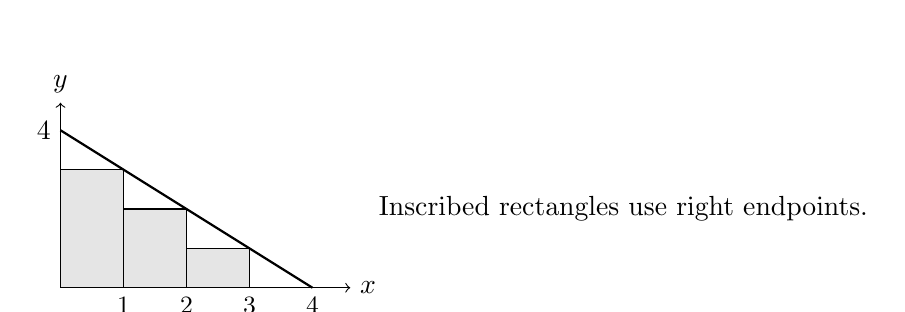
\begin{tikzpicture}[x=0.8cm,y=0.5cm]
\foreach \i in {0,1,2,3}{\pgfmathsetmacro{\h}{3-\i}
\draw[fill=gray!20] (\i,0) rectangle ({\i+1},\h);}
\draw[->](0,0)--(4.6,0) node[right]{$x$};
\draw[->](0,0)--(0,4.7) node[above]{$y$};
\draw[thick](0,4)--(4,0);
\foreach \x in {1,2,3,4}{\node[below]at(\x,0){\small$\x$};}
\node[left]at(0,4){$4$};
\node[right]at(4.9,2){Inscribed rectangles use right endpoints.};
\end{tikzpicture}
\end{center}
\item Now $\Delta x=2/n$ and $f=x^2$ is increasing, so left gives lower and right gives upper:
\begin{align*}
\ell_n&=\frac2n\sum_{i=1}^n\left(\frac{2(i-1)}n\right)^2
=\frac8{n^3}\frac{(n-1)n(2n-1)}6
=\boxed{\frac83-\frac4n+\frac4{3n^2}},\\
U_n&=\frac2n\sum_{i=1}^n\left(\frac{2i}n\right)^2
=\frac8{n^3}\frac{n(n+1)(2n+1)}6
=\boxed{\frac83+\frac4n+\frac4{3n^2}}.
\end{align*}
\item Terms containing $1/n$ or $1/n^2$ tend to zero, so both limits are $\boxed{8/3}$.
The area lies between these lower and upper sums for every $n$; the squeeze theorem forces its value to be $\boxed{8/3}$ square units.
\item (a) Width $3/n$, sample input $2+3i/n$, interval $[2,5]$:
$\boxed{\int_2^5(1+x^2)\dx}$.

(b) Width $\pi/(2n)$, sample input $\pi i/(2n)$, interval $[0,\pi/2]$:
$\boxed{\int_0^{\pi/2}\cos x\dx}$.
\item $\Delta x=\boxed{3/n}$ and $x_i=\boxed{1+3i/n}$, so
\[
\boxed{\lim_{n\to\infty}\sum_{i=1}^n
\sqrt{3+\frac{3i}{n}}\frac3n}.
\]
The extra $2$ inside $\sqrt{x+2}$ is added to the sample input $1+3i/n$.
\item On $[0,1]$, the min/max are $0,3$; on $[1,3]$, they are $3,4$; on $[3,4]$, they are $0,3$.
\[
\ell=1(0)+2(3)+1(0)=\boxed6,\qquad
U=1(3)+2(4)+1(3)=\boxed{14}.
\]
Both endpoint sums equal $9$, not $14$. On $[1,3]$, the maximum $4$ occurs at the interior point $x=2$, whereas both endpoint heights are $3$. Neither endpoint rule is an upper sum here.
\end{enumerate}

\topic{6.4}{Fundamental Theorem of Calculus}
\begin{enumerate}
\item (a) $[x^3-x^2+x]_0^2=8-4+2=\boxed6$.

(b) $[\ln x]_1^e=1-0=\boxed1$.
These definite-integral values do not need $+C$.
\item The FTC yields $\boxed{A'(x)=\sqrt{1+x^3}}$, hence $\boxed{A'(2)=3}$.
Differentiate once more using the chain rule:
\[
\boxed{A''(x)=\frac{3x^2}{2\sqrt{1+x^3}}}.
\]
The derivative of the integrand appears only in this \emph{second} derivative.
\item (a) Substitute $t=x^3$ in the integrand and multiply by $(x^3)'$:
\[
\boxed{G'(x)=3x^2\cos(x^6)}.
\]
(b) The variable is a lower bound, so
$\boxed{H'(x)=-\ln(1+x^2)}$.
\item Both bounds move:
\[
\boxed{K'(x)=3(1+9x^2)-2x(1+x^4)}.
\]
At $x=1$, $K'(1)=3(10)-2(2)=\boxed{26}$.
The lower-bound contribution must be subtracted, including its chain factor.
\item By the FTC, $F'(x)=x^2-4=(x-2)(x+2)$ and $F''(x)=2x$.
\[
\begin{array}{c|ccc}
x&(-3,-2)&(-2,2)&(2,3)\\\hline
F'(x)&+&-&+\\
F&\text{increasing}&\text{decreasing}&\text{increasing}
\end{array}
\]
Thus an interior local \textbf{maximum} occurs at $\boxed{x=-2}$ ($+$ to $-$), and an interior local \textbf{minimum} at $\boxed{x=2}$ ($-$ to $+$).
Since $F''=2x$, $F$ is concave down on $\boxed{(-3,0)}$ and concave up on $\boxed{(0,3)}$.
If values are desired, $F(x)=x^3/3-4x$, giving $F(-2)=16/3$ and $F(2)=-16/3$.
\item Net mass change:
\[
\int_0^4(2t-3)\,dt=[t^2-3t]_0^4=\boxed{4\text{ g}}.
\]
Therefore $\boxed{m(4)=10+4=14\text{ g}}$.
The derivative $m'=2t-3$ is negative before $t=3/2$ and positive after, so the mass is smallest at $\boxed{t=3/2\text{ min}}$.
\end{enumerate}

\topic{6.6}{Numerical Integration: Approximations}
\begin{enumerate}
\item The width is $h=1$; endpoint values are $0,1,4$ and midpoint values are $1/4,9/4$.
\begin{align*}
L_2&=1(0+1)=\boxed1 &&\text{low},\\
R_2&=1(1+4)=\boxed5 &&\text{high},\\
M_2&=1(1/4+9/4)=\boxed{5/2} &&\text{low},\\
T_2&=\tfrac12[0+2(1)+4]=\boxed3 &&\text{high},\\
S_2&=\tfrac13[0+4(1)+4]=\boxed{8/3} &&\text{exact}.
\end{align*}
Comparison is with $I=8/3$. The rectangle error directions follow from increasing behavior; midpoint/trapezoidal directions follow from concavity up. Simpson is exact here because the integrand is a quadratic.
\item The widths are $1,2,3$:
\[
T=\frac12(2+4)+\frac22(4+3)+\frac32(3+5)
=3+7+12=\boxed{22\text{ liters}}.
\]
Using a single common width would ignore the actual observation times.
\item Because $f'<0$, $f$ decreases:
\[\boxed{L_n\text{ over},\ R_n\text{ under}}.\]
Because $f''>0$, $f$ is concave up:
\[\boxed{M_n\text{ under},\ T_n\text{ over}}.\]
A decreasing function can still be concave up; these are distinct properties.
\end{enumerate}

\subsection*{A useful correction routine}
For each approximation, check these in order:
\begin{enumerate}[label=\arabic*.]
\item Did I count intervals rather than data points?
\item Did I use the right widths and sample inputs?
\item Did I use the rule's correct weights and outside factor?
\item Does a justified under/over comparison agree with my arithmetic?
\item Did I distinguish the approximation from its error bound?
\end{enumerate}
The remaining solutions continue on the next page.

\topic{6.6}{Numerical Integration: Error Bounds}
\begin{enumerate}[start=4]
\item For $f=x^4$ on $[0,1]$,
\[
f'=4x^3,\quad f''=12x^2,\quad f^{(4)}=24.
\]
Thus the sharp derivative bounds are $\boxed{K_1=4,\ K_2=12,\ K_4=24}$.
With $b-a=1$ and $n=4$:
\begin{align*}
E_L,E_R&\le\frac{4(1)^2}{2(4)}=\boxed{\frac12},\\
E_M&\le\frac{12(1)^3}{24(4)^2}=\boxed{\frac1{32}},\\
E_T&\le\frac{12(1)^3}{12(4)^2}=\boxed{\frac1{16}},\\
E_S&\le\frac{24(1)^5}{180(4)^4}=\boxed{\frac1{1920}}.
\end{align*}
These are guaranteed upper bounds, not claims that the actual errors equal them.
\item (a) Trapezoidal:
\[
E_T\le\frac{3(2)^3}{12n^2}=\frac2{n^2}\le0.001
\quad\Longrightarrow\quad n^2\ge2000.
\]
Since $44^2=1936<2000$ and $45^2=2025\ge2000$, the smallest certified choice is $\boxed{n=45}$.

(b) Simpson:
\[
E_S\le\frac{10(2)^5}{180n^4}=\frac{16}{9n^4}\le0.001
\quad\Longrightarrow\quad n^4\ge\frac{16000}{9}.
\]
The smallest integer satisfying the inequality is $7$, but Simpson requires an even number of intervals. Since $6^4=1296<16000/9$ and $8^4=4096>16000/9$, choose $\boxed{n=8}$.
The phrase ``smallest certified'' refers to these bounds; the unknown actual error might be smaller.
\item (a) $I\in[2.4-0.03,2.4+0.03]=\boxed{[2.37,2.43]}$.

(b) Actual absolute error is $\boxed{|2.38-2.4|=0.02}$.
The percent error is
\[
100\frac{0.02}{2.38}=\frac{100}{119}\%\approx\boxed{0.840\%}.
\]
(c) A guarantee is an inequality, $|I-Q|\le0.03$, not an equality. Here the actual error $0.02$ is smaller than the allowed maximum.
\end{enumerate}

\topic{7.1}{Slope Fields and Euler's Method}
\begin{enumerate}[itemsep=0.55em]
\item Substitute both coordinates into $x+y$:
\[
\begin{array}{c|rrr}&x=-1&x=0&x=1\\\hline
y=1&0&1&2\\y=0&-1&0&1\\y=-1&-2&-1&0\end{array}
\]
\begin{center}
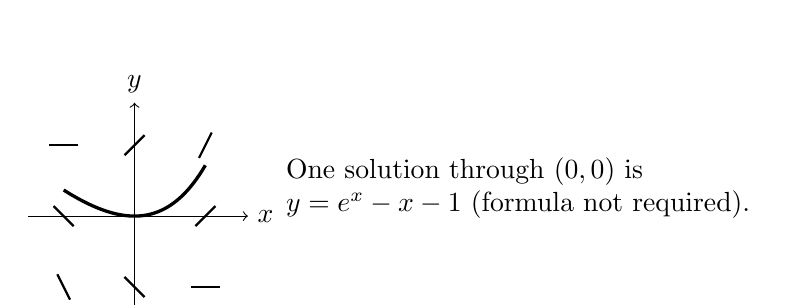
\begin{tikzpicture}[scale=0.9]
\draw[->](-1.5,0)--(1.6,0) node[right]{$x$};
\draw[->](0,-1.4)--(0,1.6) node[above]{$y$};
\foreach \x in {-1,0,1}{\foreach \y in {-1,0,1}{
\pgfmathsetmacro{\m}{\x+\y}\pgfmathsetmacro{\d}{0.2/sqrt(1+\m*\m)}
\draw[thick]({\x-\d},{\y-\m*\d})--({\x+\d},{\y+\m*\d});}}
\draw[very thick,domain=-1:1,samples=50] plot(\x,{exp(\x)-\x-1});
\node[right,align=left] at (2,0.4){One solution through $(0,0)$ is\\$y=e^x-x-1$ (formula not required).};
\end{tikzpicture}
\end{center}
The slope at $(0,0)$ is $\boxed0$, but the solution is \textbf{not constant}: the candidate $y=0$ would have derivative $0$ while the equation requires $y'=x$ there. The sketched solution has a horizontal tangent and a local minimum at the origin.
\item $\boxed{y'=2-y}$ matches all three features. It is independent of $x$, so slopes repeat along rows; $2-y$ has the required signs. The equilibrium is $\boxed{y=2}$ since its slope is zero for every $x$.
\item With $h=0.5$:
\[
\begin{array}{c|c|c|c}
x_k&y_k&x_k+y_k&y_{k+1}\\\hline
0&1&1&1+0.5(1)=1.5\\
0.5&1.5&2&1.5+0.5(2)=2.5
\end{array}
\]
Thus $\boxed{y(1)\approx2.5}$.
\item $h=(0-1)/2=\boxed{-0.5}$.
\[
\begin{array}{c|c|c|c}
x_k&y_k&x_k-y_k&y_{k+1}\\\hline
1&2&-1&2+(-0.5)(-1)=2.5\\
0.5&2.5&-2&2.5+(-0.5)(-2)=3.5
\end{array}
\]
Thus $\boxed{y(0)\approx3.5}$.
\item (a) The updates are $0+0.5(2)=1$, then $1+0.5(1)=1.5$, then $1.5+0.5(0.5)=\boxed{1.75\approx y(1.5)}$.

(b) $y''=-y'=-(2-y)=\boxed{y-2}$. This is negative while $y<2$, so the solution is concave down there.
\item (a) One step: $1+1(1)=\boxed2$.
(b) Two steps: $1+0.5(1)=1.5$, then $1.5+0.5(1.5)=\boxed{2.25}$.
(c) Both are below $e$. The absolute errors are approximately $0.71828$ and $0.46828$, respectively, so \textbf{two half-steps are closer}.
\end{enumerate}

\topic{7.2}{Antiderivatives by Substitution}
\begin{enumerate}[itemsep=0.65em]
\item (a) $u=x^2+5$, $du=2x\,dx$:
$\int u^4\,du=u^5/5+C=\boxed{(x^2+5)^5/5+C}$.

(b) $u=3x+1$, $du=3\,dx$:
$\int\cos u\,du=\boxed{\sin(3x+1)+C}$.
\item (a) $u=x^2+9$, $du=2x\,dx$:
\[
\frac12\int\frac1u\,du=\boxed{\frac12\ln(x^2+9)+C}.
\]
No absolute-value bars are needed because $x^2+9>0$.

(b) $u=1+e^x$, $du=e^x\,dx$:
$\boxed{\ln(1+e^x)+C}$; again the input to the logarithm is positive.
\item (a) $u=2+\cos x$, $du=-\sin x\,dx$:
\[
-\int u^{-1/2}\,du=-2u^{1/2}+C
=\boxed{-2\sqrt{2+\cos x}+C}.
\]
(b) $u=3x^2$, $du=6x\,dx$, and $9x^4=u^2$:
\[
\int\frac{1}{1+u^2}\,du=\boxed{\arctan(3x^2)+C}.
\]
\item $u=x^2+5$, $du=2x\,dx$; the limits $x=0,2$ become $u=5,9$:
\[
\int_0^2x\sqrt{x^2+5}\dx
=\frac12\int_5^9u^{1/2}\,du
=\left[\frac{u^{3/2}}3\right]_5^9
=\boxed{\frac{27-5\sqrt5}{3}}.
\]
\item Let $u=x^2$, $du=2x\,dx$. Then $F=e^{x^2}+C$.
From $F(0)=3$, $1+C=3$, so $\boxed{F(x)=e^{x^2}+2}$.
Check: $F'=2xe^{x^2}$ and $F(0)=1+2=3$.
\item (a) Differentiating by the product or quotient rule gives
\[
\frac{d}{dx}\left(\frac{\sin(x^2)}{2x}\right)
=\cos(x^2)-\frac{\sin(x^2)}{2x^2}.
\]
The extra term means the claim is false.

(b) $u=x^2$ gives $du=2x\,dx$, but the integrand has no $x$ factor to absorb. Dividing an antiderivative by a variable is not a valid reverse-chain-rule shortcut.

(c) In the related integral, the needed factor \emph{is} present:
\[
\int x\cos(x^2)\dx=\frac12\int\cos u\,du
=\boxed{\frac12\sin(x^2)+C}.
\]
\end{enumerate}
\end{document}
